\begin{figure}
    \centering
    %\vspace{-1em}
    \begin{subfigure}[b]{0.49\linewidth} % 40% width
        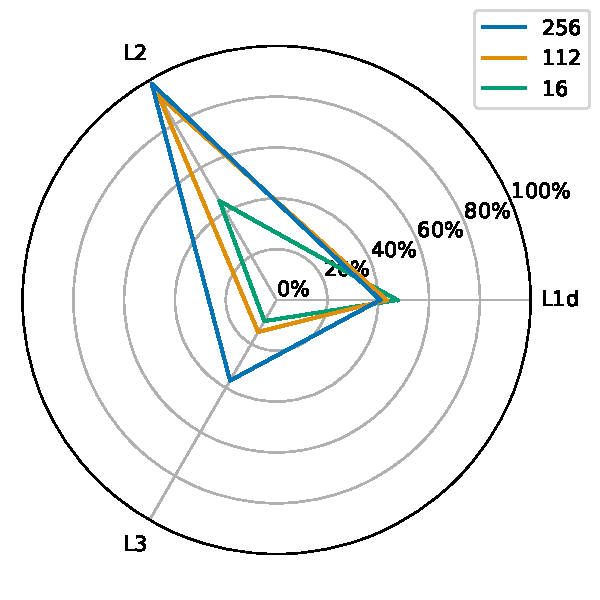
\includegraphics[width=\linewidth]{img_misses_proteins.pdf}
        \vspace{-2.2em}
        \caption{\texttt{proteins}}
        %\vspace{0.5em}
        \label{fig:miss-proteins}
    \end{subfigure}
    \begin{subfigure}[b]{0.49\linewidth} % 40% width
        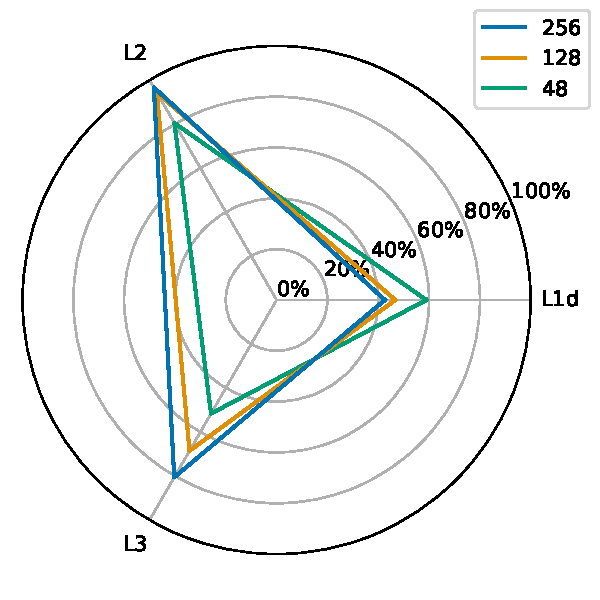
\includegraphics[width=\linewidth]{img_misses_arxiv.pdf}
        \vspace{-2.2em}
        \caption{\texttt{arxiv}}
        %\vspace{0.5em}
        \label{fig:miss-arxiv}
    \end{subfigure}
    \begin{subfigure}[b]{0.49\linewidth} % 40% width
        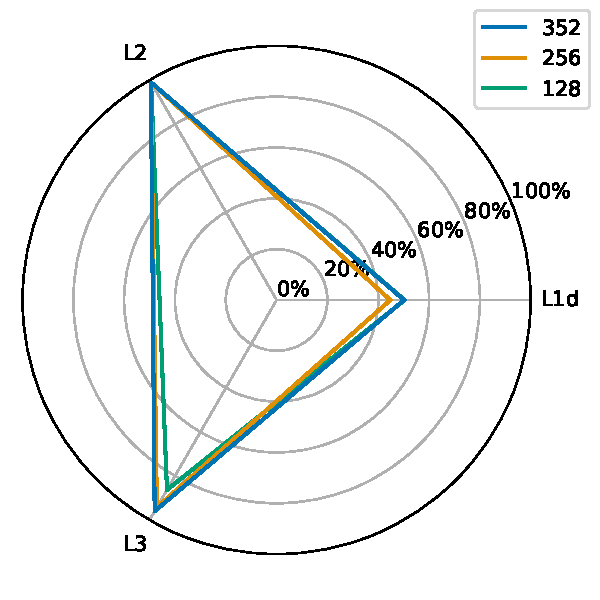
\includegraphics[width=\linewidth]{img_misses_mag.pdf}
        \vspace{-2.2em}
        \caption{\texttt{mag}}
        %\vspace{0.5em}
        \label{fig:miss-mag}
    \end{subfigure}
    \begin{subfigure}[b]{0.49\linewidth} % 40% width
        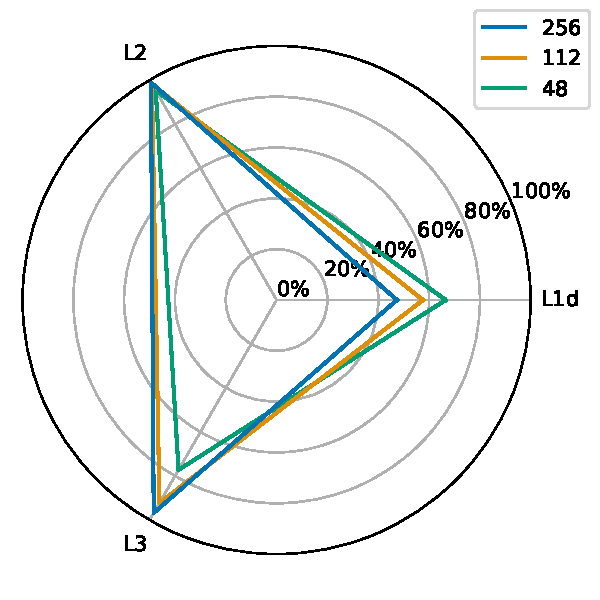
\includegraphics[width=\linewidth]{img_misses_products.pdf}
        \vspace{-2.2em}
        \caption{\texttt{products}}
        %\vspace{0.5em}
        \label{fig:miss-products}
    \end{subfigure}
    %\vspace{-1em}
    \caption[Cache miss rate for embedding lookups on CPU.]{Cache miss rate for GNN embedding lookups on the multicore CPU baseline. Each subfigure reports one input graph, and each line corresponds to one embedding-vector size. The radar axes report the L1D, L2, and L3 miss rates, computed as the percentage of vector requests that miss at each cache level. The high-locality graphs, \texttt{proteins} and \texttt{arxiv}, show substantially lower L3 miss rates because repeated accesses to nearby embedding vectors allow the LLC to filter many requests. In contrast, \texttt{mag} and \texttt{products} remain close to the outer rings for L2 and L3, indicating that most vector lookups continue to lower cache levels or HBM. Larger embedding vectors generally reduce L1D miss rates by exposing more spatial locality within each vector, but increase pressure on L2 and L3 because each cached vector occupies more capacity. Thus, L3 miss rates range from 38\% to 92\% across inputs and embedding sizes, showing that cache effectiveness depends strongly on graph locality and vector size.}
    \label{fig:misses}
\end{figure}
